\newcommand{\printlayout}{%
\node (L1) {};
\node[right of=L1] (L2) {};
\node[right of=L2] (L3) {};
\node[right of=L3] (L4) {};
\node[below of=L1] (R1) {};
\node[right of=R1] (R2) {};
\node[right of=R2] (R3) {};
\node[right of=R3] (R4) {};}
\begin{tabular}{rccc}
     & & $B(0)$ & $B(1)$ \\
     & - & \boxed{\scalebox{0.3}{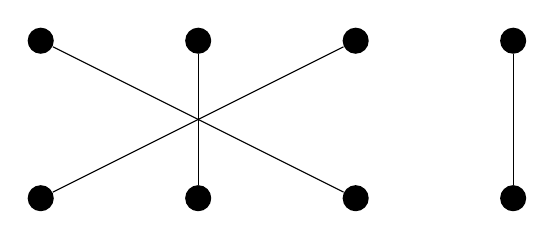
\begin{tikzpicture}[node distance=20mm, auto, every node/.append style={circle, draw=none, fill=black}]
    \printlayout
    \draw (L1) -- (R3);
    \draw (L2) -- (R2);
    \draw (L3) -- (R1);
    \draw (L4) -- (R4);
    \end{tikzpicture}}} & 
    \boxed{\scalebox{0.3}{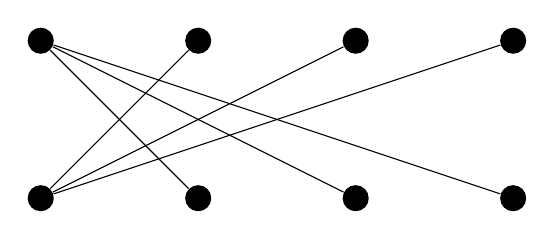
\begin{tikzpicture}[node distance=20mm, auto, every node/.append style={circle, draw=none, fill=black}]
    \printlayout
    \draw (L1) -- (R2);
    \draw (L1) -- (R3);
    \draw (L1) -- (R4);
    \draw (R1) -- (L2);
    \draw (R1) -- (L3);
    \draw (R1) -- (L4);    
    \end{tikzpicture}}}\\
    $A(0)$ & \boxed{\scalebox{0.3}{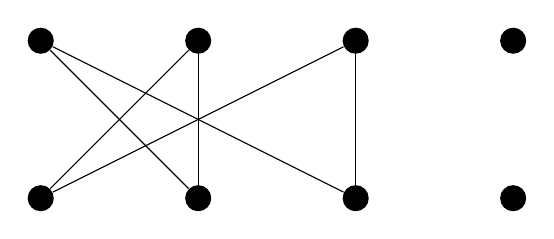
\begin{tikzpicture}[node distance=20mm, auto, every node/.append style={circle, draw=none, fill=black}]
    \printlayout
    \draw (L1) -- (R2);
    \draw (L1) -- (R3);
    \draw (L2) -- (R1);
    \draw (L2) -- (R2);
    \draw (L3) -- (R3);
    \draw (L3) -- (R1);
    \end{tikzpicture}}} & 
    \boxed{\scalebox{0.3}{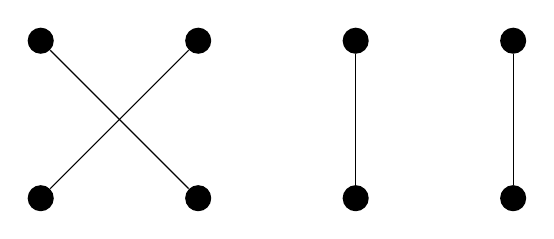
\begin{tikzpicture}[node distance=20mm, auto, every node/.append style={circle, draw=none, fill=black}]
    \printlayout
    \draw (L1) -- (R2);
    \draw (L2) -- (R1);
    \draw (L3) -- (R3);
    \draw (L4) -- (R4);
    \end{tikzpicture}}}& 
    \boxed{\scalebox{0.3}{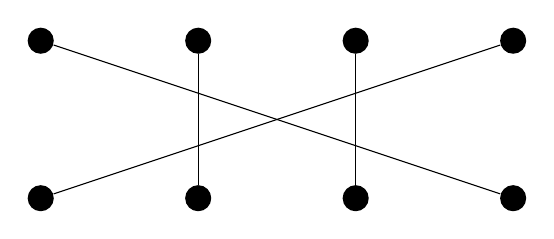
\begin{tikzpicture}[node distance=20mm, auto, every node/.append style={circle, draw=none, fill=black}]
    \printlayout
    \draw (L1) -- (R4);
    \draw (L2) -- (R2);
    \draw (L3) -- (R3);
    \draw (L4) -- (R1);
    \end{tikzpicture}}}\\
    $A(1)$ & \boxed{\scalebox{0.3}{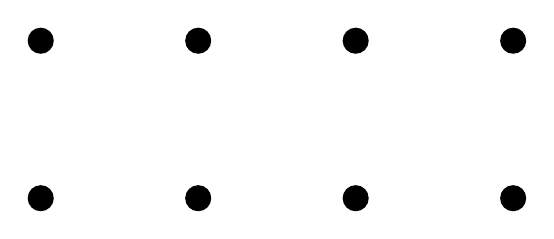
\begin{tikzpicture}[node distance=20mm, auto, every node/.append style={circle, draw=none, fill=black}]
    \printlayout
    \end{tikzpicture}}} & \boxed{\scalebox{0.3}{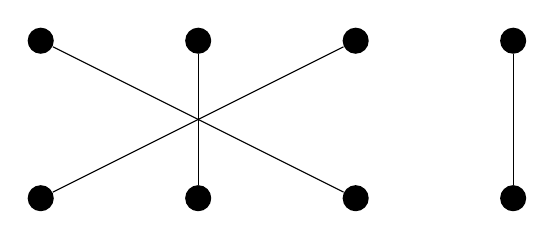
\begin{tikzpicture}[node distance=20mm, auto, every node/.append style={circle, draw=none, fill=black}]
    \printlayout
    \draw (L1) -- (R3);
    \draw (L2) -- (R2);
    \draw (L3) -- (R1);
    \draw (L4) -- (R4);
    \end{tikzpicture}}} & 
    \boxed{\scalebox{0.3}{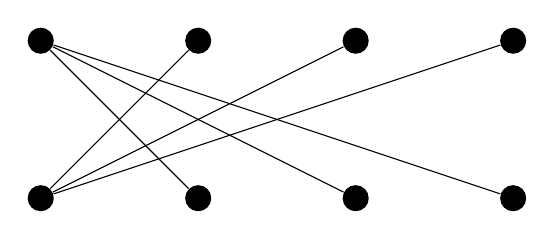
\begin{tikzpicture}[node distance=20mm, auto, every node/.append style={circle, draw=none, fill=black}]
    \printlayout
    \draw (L1) -- (R2);
    \draw (L1) -- (R3);
    \draw (L1) -- (R4);
    \draw (R1) -- (L2);
    \draw (R1) -- (L3);
    \draw (R1) -- (L4);    
    \end{tikzpicture}}} \\
\end{tabular}
